% This must be in the first 5 lines to tell arXiv to use pdfLaTeX, which is strongly recommended.
\pdfoutput=1
% In particular, the hyperref package requires pdfLaTeX in order to break URLs across lines.

\documentclass[11pt]{article}

% Change "review" to "final" to generate the final (sometimes called camera-ready) version.
% Change to "preprint" to generate a non-anonymous version with page numbers.
% \usepackage[final]{acl}
\usepackage[review]{acl}

% Standard package includes
\usepackage{times}
\usepackage{latexsym}
\usepackage{graphicx}
\usepackage{amsmath}
\usepackage{amsfonts}
% For proper rendering and hyphenation of words containing Latin characters (including in bib files)
\usepackage[T1]{fontenc}
% For Vietnamese characters
% \usepackage[T5]{fontenc}
% See https://www.latex-project.org/help/documentation/encguide.pdf for other character sets



% This assumes your files are encoded as UTF8
\usepackage[utf8]{inputenc}
\usepackage{CJKutf8}
\usepackage{subcaption}
\usepackage{hyperref}

% This is not strictly necessary, and may be commented out,
% but it will improve the layout of the manuscript,
% and will typically save some space.
\usepackage{microtype}
\usepackage{lscape}

% This is also not strictly necessary, and may be commented out.
% However, it will improve the aesthetics of text in
% the typewriter font.
\usepackage{inconsolata}
\usepackage{xcolor}
\usepackage{tipa}
\usepackage{multirow}
\usepackage{array}


\newcommand{\MY}[1]{\textcolor{blue}{(Mengyue: #1)}}
\newcommand{\KZ}[1]{\textcolor{red}{(Kenny: #1)}}
\newcommand{\HA}[1]{\textcolor{brown}{(Haoan: #1)}}
\newcommand{\YV}[1]{\textcolor{magenta}{(Yvonne: #1)}}
\newcommand{\XJ}[1]{\textcolor{orange}{(Xiujie: #1)}}
\newcommand{\secref}[1]{Sec. \ref{#1}}
\newcommand{\figref}[1]{Figure \ref{#1}}
\newcommand{\eqnref}[1]{Eq. (\ref{#1})}
\newcommand{\tabref}[1]{Table \ref{#1}}
\newcommand{\exref}[1]{Example \ref{#1}}
\newcommand{\appref}[1]{Appendix \ref{#1}}

% If the title and author information does not fit in the area allocated, uncomment the following
%
%\setlength\titlebox{<dim>}
%
% and set <dim> to something 5cm or larger.

\title{Automatic Reconstruction of Ancient Chinese Pronunciations}

% Author information can be set in various styles:
% For several authors from the same institution:
% \author{Author 1 \and ... \and Author n \\
%         Address line \\ ... \\ Address line}
% if the names do not fit well on one line use
%         Author 1 \\ {\bf Author 2} \\ ... \\ {\bf Author n} \\
% For authors from different institutions:
% \author{Author 1 \\ Address line \\  ... \\ Address line
%         \And  ... \And
%         Author n \\ Address line \\ ... \\ Address line}
% To start a separate ``row'' of authors use \AND, as in
% \author{Author 1 \\ Address line \\  ... \\ Address line
%         \AND
%         Author 2 \\ Address line \\ ... \\ Address line \And
%         Author 3 \\ Address line \\ ... \\ Address line}

\author{First Author \\
  Affiliation / Address line 1 \\
  Affiliation / Address line 2 \\
  Affiliation / Address line 3 \\
  \texttt{email@domain} \\\And
  Second Author \\
  Affiliation / Address line 1 \\
  Affiliation / Address line 2 \\
  Affiliation / Address line 3 \\
  \texttt{email@domain} \\}

\begin{document}
\maketitle
\begin{abstract}

This paper attempts to discover communication patterns automatically within dog vocalizations
in a data-driven approach, which breaks the barrier previous approaches that rely
on human prior knowledge on limited data. 
We present a self-supervised approach with HuBERT, enabling the accurate classification 
of phones, and an adaptive grammar induction method that identifies phone sequence patterns 
that suggest a preliminary vocabulary within dog vocalizations. 
Our results show that a subset of this vocabulary has substantial causality relations
with certain canine activities, suggesting signs of stable semantics associated with these
``words''.
%We use this approach to undercover phonemes and mine vocabulary of dogs. 
%We further develop a web-based dog vocalization labeling system. This system can highlight phoneme n-grams, present in the vocabulary, in the dog audio uploaded by users.
%This approach can be simply applied to find other non-human language sound units and is valuable for further research on dog language understanding.

\end{abstract}

\section{Introduction}
\label{sec:intro}

Evaluation of dialogue systems is an open problem. Existing
automatic evaluation metrics for chitchat systems are similar to those for 
other text generation tasks (e.g., machine translation \citep{papineni-etal-2002-bleu}, question-answering \citep{rajpurkar-etal-2016-squad}, 
summarization \citep{lin-2004-rouge}), which depends on calculating word 
overlaps with reference responses. 
However, for chitchats, there are usually 
many alternative but plausible responses given a situation, 
perhaps more than any other text generation task mentioned above. 
A limited number of reference responses are 
not sufficient to determine how good a generated response is. 
Moreover, such static settings are not good at
assessing an interactive, context-sensitive system.

Interactive human evaluation metrics usually 
involve a Likert scale evaluation after a multi-turn conversation 
with the bot to be assessed. 
While this method is a step up from the previous static evaluation, 
it is difficult for human judges to give a concrete score to
any bot.
%\KZ{But are we also asking judges to score invidividual bots, which is difficult?} 
Comparing the performance of two bots is easier. 
Thus ACUTE-EVAL~\citep{DBLP:journals/corr/abs-1909-03087} asks the 
judges to make a binary judgment of who is better in conversations between two identical bots 
or between a human and a bot. A more advanced version of that
is \textit{Spot The Bot}~\cite{deriu-etal-2020-spot} which models the 
human evaluation of a 
conversation after the Turing test. However, such a process is still 
time-consuming and costly, compared with automatic evaluations.

In our opinion, a good method for evaluating multi-turn 
conversational model/system 
should satisfy the following requirements:
i) be as efficient and inexpensive as possible;
ii) can truly reflect a model's ability to conduct a human conversation; 
iii) evaluation results should correlate well with human judgments;
iv) can be used to compare and rank the capabilities of a set of models/systems.
  
Toward that goal, in this work, we propose an automatic interactive evaluation 
framework, which is called \textit{ChatMatch}(CM) for chitchat
agents. This framework can be used to rank a number of bots with little
time and minimum human effort.  Above all, we want to emphasize 
the significance of direct interactions between bots 
in the evaluation.
%\textcolor{red}{Reviewer 1 said that he didn't understand this sentence. Maybe remove "the observation"?} 
People tend to believe that human-bot conversations are more reliable 
and produce more comprehensive evaluations of chatbots' capabilities. 
This is not always true. As human annotators know their counterpart is a robot, 
they tend to ask common and goal-directed questions. 
On the other hand, some bot-bot chat logs in our experiments show that, 
surprisingly, conversations between different bots may expose their strengths 
and weaknesses never seen in human-bot conversations. 
\figref{fig:two convs} gives two small chat fragments, illustrating such
differences.
While talking about hobbies, human keeps asking the bot some blunt
questions, which leads to dull responses from the bot.
However, in a bot-bot setting, two bots, including the same bot in the previous
conversation, start explaining their hobbies to each other, producing a more
interesting conversation. 

\begin{figure}[ht!]
 \centering

% \subfigure[Chat snippet between human and bot (Plato-2)]{
\subfigure[Chat snippet between human and bot]{ 
 %  \centering
  %  \begin{minipage}[t]{0.5\linewidth}
  \includegraphics[width=0.95\linewidth]{eg4.eps}\label{fig:sub-first}
  %  \end{minipage}
 }
 
 \subfigure[Chat snippet between two bots]{
  % \centering
  % \begin{minipage}[t]{0.5\linewidth}
  \includegraphics[width=0.95\linewidth]{figs.eps}\label{fig:sub-second}
  % \end{minipage}
 }
 \caption{Snippets from human-bot and bot-bot chat logs}
\label{fig:two convs}
\end{figure}

Our framework consists of two components: \textit{competition} and 
\textit{scoring}, which interoperate with each other. 
The competition is modeled
after most sports tournaments such as soccer or ping pong. 
There are three levels of competitions. From bottom up, they are:
game-level, match-level and tournament-level. 
Each match consists of several games. During a game, two bots will converse 
freely with each other and a virtual judge will score their performances 
according to a set of user-defined criteria such as consistency and fluency, 
etc.  These criteria are flexible and extensible.
%As an example like \figref{fig:example} shows, 
%Bot $A$ will be 
%penalized twice for repeating while Bot $B$ will be penalized once for 
%contradicting itself. In addition to the penalty, 
%a bonus point is rewarded to $A$
%who shows to produce relevant response with long term memory. 
%\KZ{Do we still have this as a criterion?}
%However, the specific bonus and penalty settings may vary 
%depending on the domain and scenarios that the experiment is 
%set in. 

%\begin{figure}[th!]
%	\centering
%	\includegraphics[width=0.95\columnwidth]{example.eps}
%	\caption{A chat snippet between two bots.}
%	\label{fig:example}
%\end{figure}

The main contributions of this paper are:
\begin{itemize}
\item We propose the first interactive evaluation framework for chatbots which
is based solely on bot-bot conversations and modeled after sports competitions (\secref{sec:competition}).
\item We designed three algorithms to score \textit{diversity}, \textit{consistency}, \textit{relevance}, three important dimensions in a bot's chatting 
abilities.
\item  The entire scoring process is fully automated and efficient. 
In our experiments, the system can rank seven bots in less than 
three minutes on average (\secref{sec:scoring}, \secref{sec:time}).
\item  Our experiments show that the results produced by our framework
closely correlate with the human evaluation results. 
Results also show that our framework outperforms 
several recent strong baseline evaluation systems (\secref{sec:main}).
%\item %We demonstrate the improvements in efficiency 
%using direct chat logs between bots.
%\KZ{Maybe this should not be a contribution but part of the conclusion?}
%We show that the chats between bots are impressively informative, 
%even richer than the chats between humans and bots.
%This suggests some possible directions to improve 
%the capabilities of bots in the future.
%(e.g., by having them learn from each other)  (\secref{sec:diversity})
\end{itemize}

\section{ACP Dataset Construction}\label{sec:dataset}
% When reconstructing the phonetic system, Wang always follows the taxonomy in \textit{Qieyun} and attach pronunciations, represented by phonetic symbols, onto each initial or final category based on \textit{Qieyun} taxonomy. This reconstruction makes use of contemporaneous written materials, primarily poetic and literary materials since these works often have rigorous rhyming rule, thus similarities among certain categories, especially for syllable finals, can be deduced.
% \MY{You wanna name your dataset? i.e. AncientChinesePhones (ACP), things like this}
% \MY{Can you use 1 sentence to say why we need to combine them? like if following only 1 data, what would we miss?}
Our \textbf{ACP} (Ancient Chinese Pronunciation) dataset offers character-wise chronological data of ancient Chinese pronunciation, combining two kinds of data: the digitized \textit{Guangyun} data \cite{kanji_database_project__2004} and the phonological reconstruction result of \citet{wang_l_hanyu_2012}. For a given character, the former informs us the category it belongs to, and the latter tells us the pronunciation reconstruction results on each category.

\textit{Guangyun} is a rhyme dictionary using a special sound annotation called \textit{Fanqie}. Chinese characters are monosyllabic, i.e. all Chinese character's pronunciation correspond to one syllable, each comprised of an initial and a final\cite{duanmu2007phonology}. According to \textit{Fanqie}, each Chinese character's pronunciation is described as a combination of two representative characters, one for its \textit{initial} and another for its \textit{final} as shown in Figure \ref{fig:fanqie}. 
    \begin{figure}[ht]
        \centering
        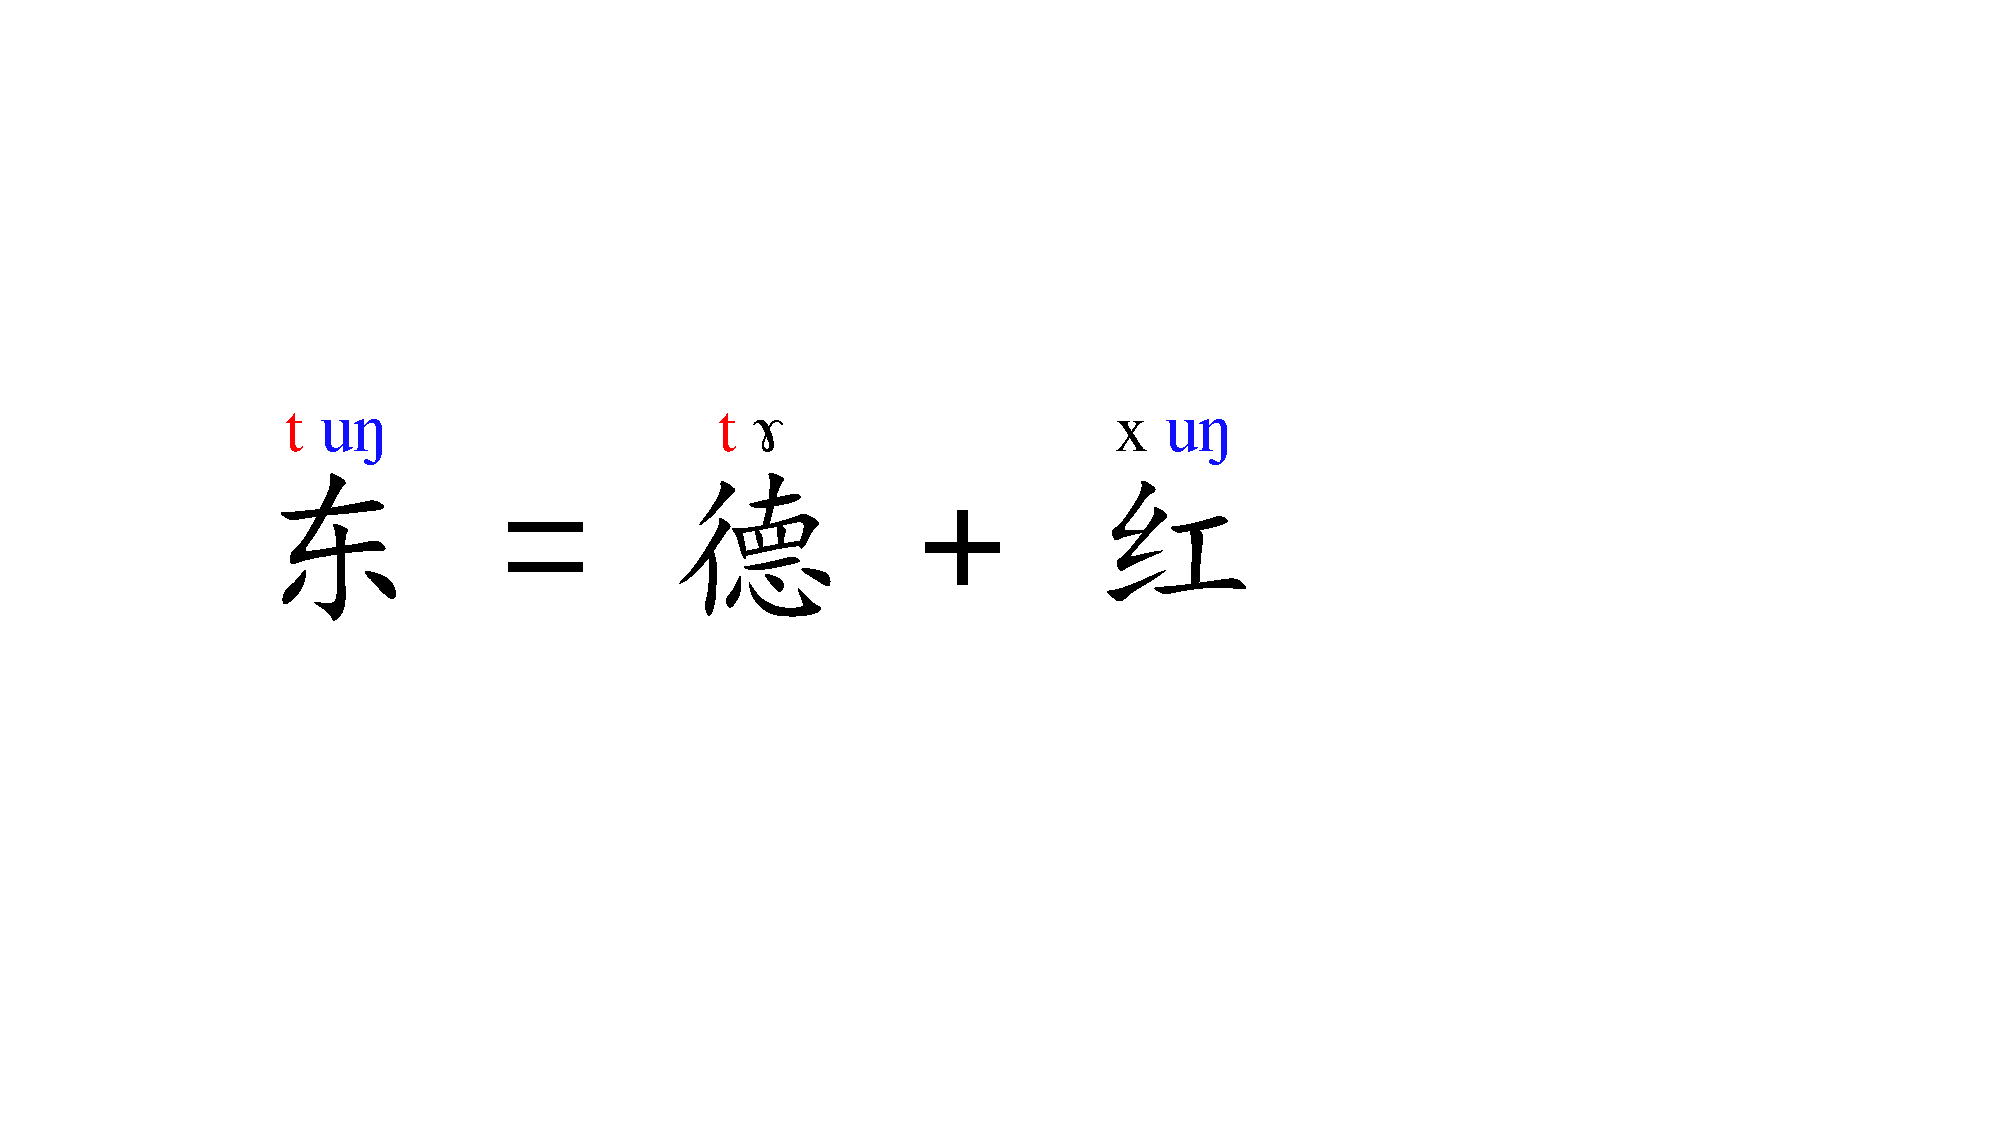
\includegraphics[width=5cm]{images/fanqie.pdf}
        \caption{Method of \textit{Fanqie}:  \begin{CJK*}{UTF8}{gbsn}“东”\end{CJK*} belongs to category \begin{CJK*}{UTF8}{gbsn}“德”\end{CJK*}(\textipa{[t]}) for initial and to category \begin{CJK*}{UTF8}{gbsn}“红”\end{CJK*}(\textipa{[uN]})for final.}
        \label{fig:fanqie}
    \end{figure}

Under this taxonomy, there are 38 categories of initials and 298 categories of finals. The aim of phonological reconstruction is to attach the exact pronunciation (denoted by IPA phoneme) onto each initial and final category for targeted period. These information can be found in \citet{wang_l_hanyu_2012}'s reconstruction results of Chinese phonology, which includes the evolution of Chinese pronunciation system from PreQin (-206 BC) to modern Chinese (AD 1912-) at 9 different representative time points. We have only selected results for 6 historical periods after that MiddleTang dynasty: \texttt{MiddleTang, LateTang, Song, Yuan, MingQing and Modern}, represented by the midpoint in time of each historical period (AD 709, AD 898, AD 1120, AD 1324, AD 1640, AD 1968), since these reconstruction results are more consistent among different linguists\cite{zuofan_1936,wang_l_hanyu_2012}. See Figure \ref{fig:timeline} for the Chinese history timeline.
% \MY{so T is for MiddleTang? These abbreviations are a bit weird, consider using ABCDE instead, as they can suggest an order. Or you can list the current abbreviations in brackets in lines 152-155 as i just did} 

When constructing ancient Chinese pronunciation for each character in ACP dataset, 4 possible cases are presented (More examples in  \appref{app:reconstruction}):

    \paragraph{Direct determination of pronunciation} 
    If the exact pronunciation is directly given for one category, then the given IPA phoneme is attached onto each character within this category. For example, \begin{CJK*}{UTF8}{gbsn}“波”\end{CJK*} belongs to initial category of \begin{CJK*}{UTF8}{gbsn}“帮”\end{CJK*} and [p] is attached to category \begin{CJK*}{UTF8}{gbsn}“帮”\end{CJK*}, then the initial IPA of \begin{CJK*}{UTF8}{gbsn}“波”\end{CJK*} is [p].
    This is the case for pronunciation system of MiddleTang since all characters strictly belongs to its category denoted in \textit{Guangyun}.

    \paragraph{Rule-based determination of pronunciation}
    If there exists several possible pronunciations for the same category,
    then the linguistic rules given by Wang are applied to help choose the correct one. Rules on initials' pronunciation are usually based on finals' category, and rules on finals' pronunciation are usually based on the articulation information recorded in \textit{Guangyun}
    \footnote{The articulation information is only vaguely recorded in \textit{Guangyun}.}. For example, \begin{CJK*}{UTF8}{gbsn}“砩”=“帮”+“废”\end{CJK*} and \begin{CJK*}{UTF8}{gbsn}“碑”=“帮”+“支”\end{CJK*} both belongs to initial category of \begin{CJK*}{UTF8}{gbsn}“帮”\end{CJK*}, but given the linguistic rule that \begin{CJK*}{UTF8}{gbsn}“帮”\end{CJK*} represents [f] only under the case when fianl category is \begin{CJK*}{UTF8}{gbsn}废\end{CJK*}, and represent [p] in other cases, we attach [f] as \begin{CJK*}{UTF8}{gbsn}砩\end{CJK*}'s initial IPA and [p] as \begin{CJK*}{UTF8}{gbsn}碑\end{CJK*}'s initial IPA.
    This is the case for LateTang and Song period since a small amount of categories' pronunciation has encountered rule-based change.
    
    \paragraph{Arbitrary determination of pronunciation}
    
    If a category-wise pronunciation reconstruction is no given due to the complexity of the language system's evolution, then we manually digitize Wang's example on several representative characters' pronunciation. This is the case for Yuan and MingQing
    % \MY{use full spelling for these dynasties in main text}
    pronunciation system since the overall categorization has significantly changed compared to MiddleTang phonology system.
    
    \paragraph{Converted pronunciation}
    For modern Chinese language system, we take Mandarin as its representative. Since Mandarin is a living language, we directly convert the pronunciation to IPA representation.

\begin{figure*}[ht]
    \centering
    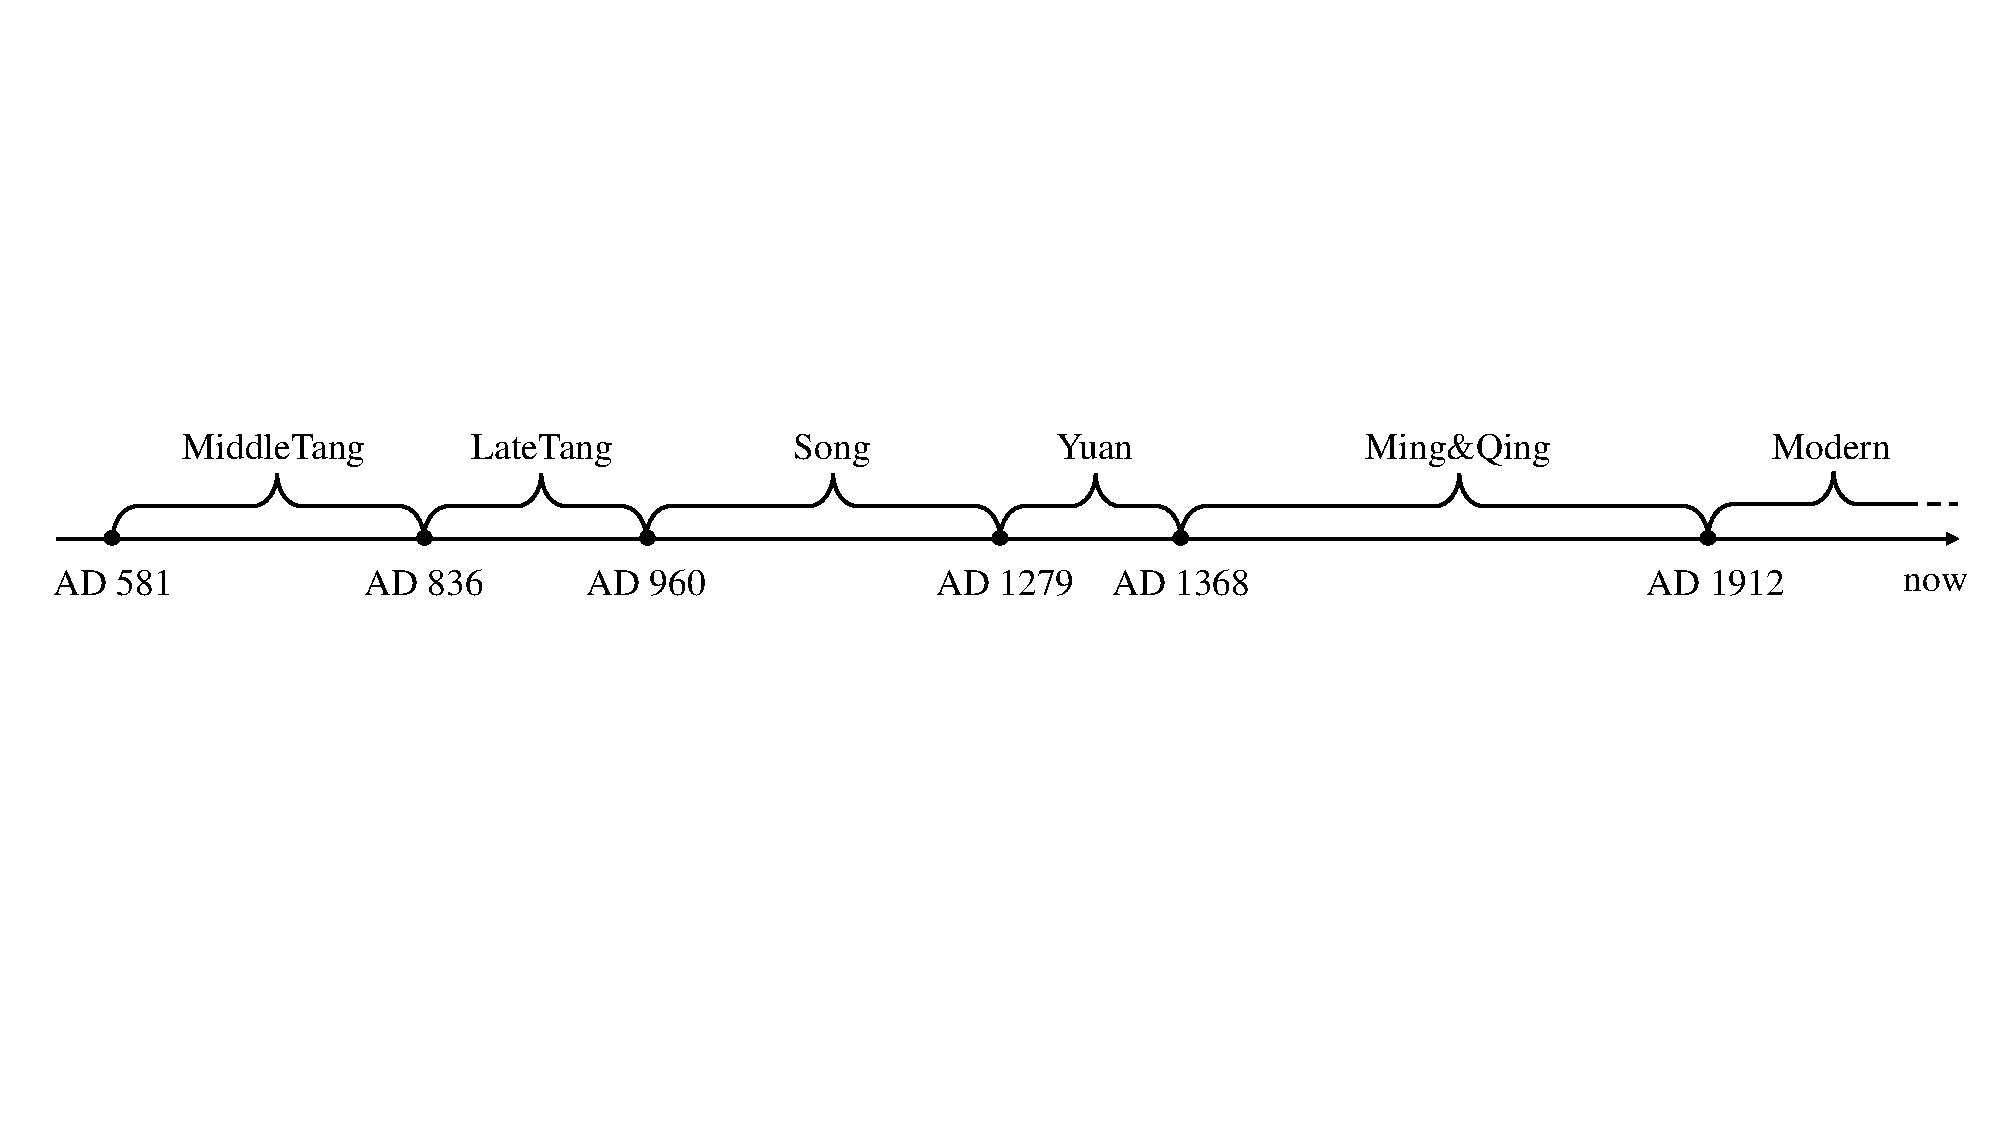
\includegraphics[width=0.9\textwidth]{images/history_tl.pdf}
    \caption{China history timeline. The 6 pronunciation systems represents the overall spoken language form in a certain period of time. 
    % \KZ{abbreviation to one letter. delete dynastie name, match result with model figure
    % Fig still very blurry when magnified. The Sui, Tang etc. below the time axis is not needed when you have the red part on the top. A dynasty should be a time period and not a point anyway. Also Republic Period should be ROC, and PRC is 1949 not 1945.}
    }
    \label{fig:timeline}
\end{figure*}

Following these IPA symbols and conditions, we manually attach the initials and finals, take all the available records as single entries and left the unknown entries blank. Meanwhile, another articulation information, the tone, is much more complicated to trace since rhyme dictionaries focus on initials' and finals' taxonomy and only give vague description on tone\cite{wang_l_hanyu_2012}. The linguistic reconstructions have no consistent results \cite{zhiping_1986_tone, xiangdong_earlytang, wuyun_1982}, thus neither encoded into ACP dataset for any of the time period. 
% \MY{need ref and a bit explanation on why tone information is difficult to trace}

According to the articulation feature, we further divide the final part into Medial, Nucleus and Coda as shown in \figref{fig:split}. The medial is an optional part of the final, usually has short and soft sounding, connecting initial and final. The nucleus is the main and non-empty vowel in final. The coda is attached to nucleus which can only be consonant or empty. Finally, each single entry in our dataset is composed of 4 parts: Initial-I, Medial-M, Nucleus-N and Coda-C, either empty (denoted by ``-") or non-empty (denoted by one IPA phoneme). Example of complete and incomplete sets of pronunciations for one character in the dataset can be found in \tabref{tab: Dataset example}. The final dataset contains 17,001 entries for each of the 17,001 Chinese characters in MiddleTang, LateTang, Song and Modern historical period\tabref{tab:dataset}. Meanwhile, only 1,402 entries for Yuan and 1,519 entries for MingQing is provided while other filled with [UNK] due to the inherent incompleteness in linguistics reconstruction.

\begin{table}[ht]
    \centering
    \footnotesize
    \begin{tabular}{l@{\hskip 4pt}c@{\hskip 4pt}c@{\hskip 4pt}c@{\hskip 4pt}c@{\hskip 4pt}c@{\hskip 4pt}c}
    \hline
     & \textbf{T} & \textbf{L} & \textbf{S} & \textbf{Y} & \textbf{Q} & \textbf{M}\\
    \hline
    \textbf{Entries} & 17,001 & 17,001 & 17,001 & 1,420 & 1,519 & 17,001\\
    \textbf{Coverage} & 100\% & 100\% & 100\% & 8.25\% & 8.93\% & 100\%\\
    \hline
    \end{tabular}
    \caption{The statistics of ACP dataset. Abbreviations: T - MiddleTang, L - LateTang, S - Song, Y - Yuan, Q - MingQing, M - Modern.}
    \label{tab:dataset}
\end{table}

\begin{figure}[h!]
    \centering
    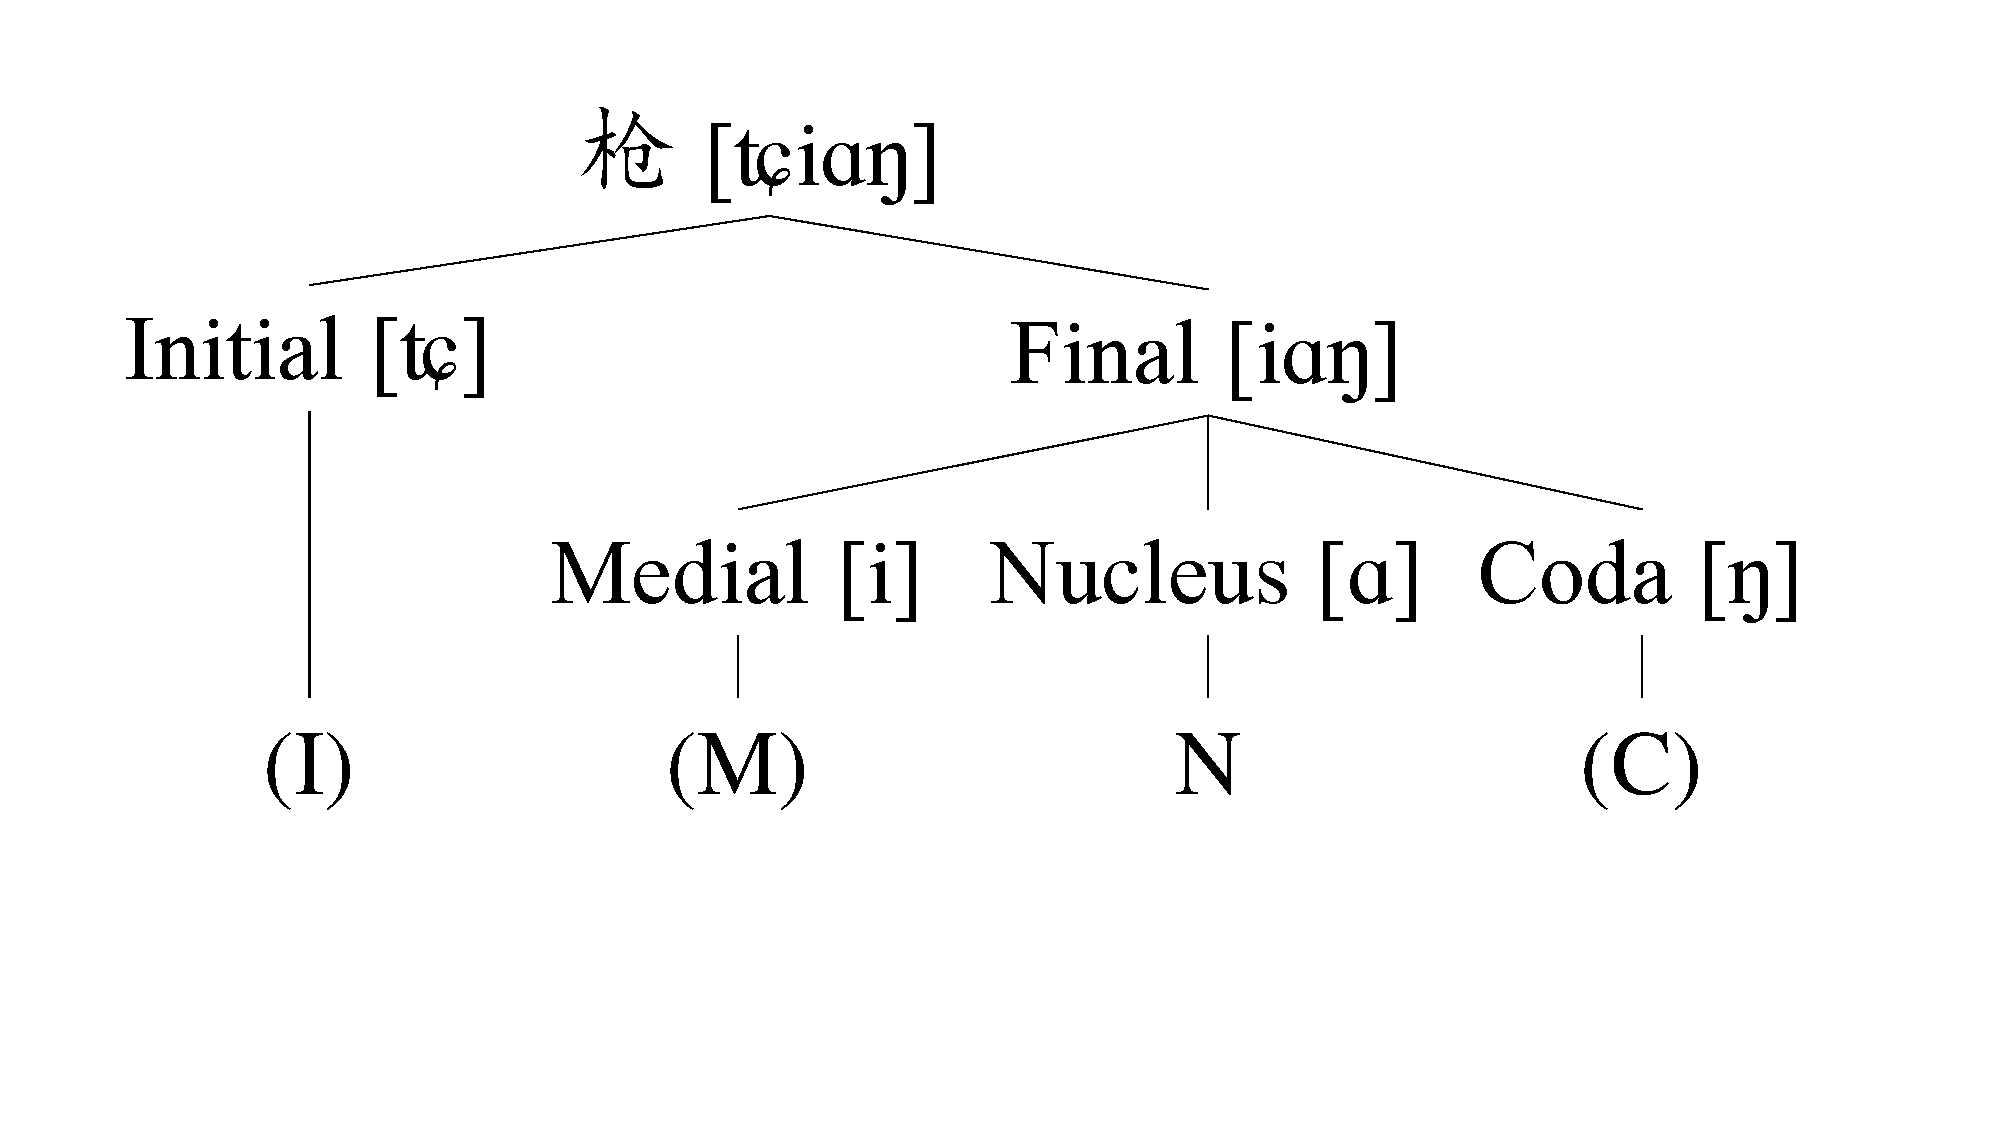
\includegraphics[width=7cm]{images/split.pdf}
    \caption{The phoneme sequence is split into initial, medial, nucleus and coda, where initial, medial and coda are optional.
    }
    \label{fig:split}
\end{figure}


\begin{table*}[ht]
    \centering
    \footnotesize
    \resizebox{\linewidth}{!}{
    \begin{tabular}{ccccccccccccccccccccccccc}
    \hline
\multicolumn{1}{c}{\multirow{2}{*}{Character}} &
  \multicolumn{4}{c}{\textbf{MiddleTang}} &
  \multicolumn{4}{c}{\textbf{LateTang}} &
  \multicolumn{4}{c}{\textbf{Song}} &
  \multicolumn{4}{c}{\textbf{Yuan}} &
  \multicolumn{4}{c}{\textbf{MingQing}} &
  \multicolumn{4}{c}{\textbf{Modern}} \\
\multicolumn{1}{c}{}&I&M&N&C& I & M & N  & C & I & M & N  & C & I & M & N  & C & I  & M & N  & C & I  & M & N  & C \\
    \hline
\begin{CJK*}{UTF8}{gbsn}纣\end{CJK*} & d & i & ou & - & \textctd & i & \textipa{@u} & - & t\textctc & i & \textipa{@u} & - & t\textctc & i & \textipa{@u} & - & \textrtails & - & \textipa{@u} & - & t\textrtails  & - & ou & - \\
\begin{CJK*}{UTF8}{gbsn}雍\end{CJK*} & \textipa{\textglotstop} & i & u & \textipa{N} & \textipa{\textglotstop} & i & u & \textipa{N} & j & i & u & \textipa{N} & \multicolumn{4}{c}{UNK} & j & - & y & \textipa{N}  & j & - & u & \textipa{N} \\
\begin{CJK*}{UTF8}{gbsn}皙\end{CJK*} & s & - & i & k & s & i & \textipa{@} & k & s & - & i & t & \multicolumn{4}{c}{UNK} & \multicolumn{4}{c}{UNK} & \textctc & - & i & - \\
    \hline
    \end{tabular}}
    \caption{Example of complete and incomplete sets in the dataset.}
    \label{tab: Dataset example}
\end{table*}

% \MY{From my perspective, our main contribution is the digital version of this ancient chinese pronunciation dataset. Hence, we'd better give a screenshot/smaller version of the dataset to showcase what you did here, including the timeline, different characters, their respective initial, nucleus and coda. Also, a link to full access of Yvonne's excel (the dataset itself, but in a visualized version and a csv/json file) is preferred. I think Yvonne maybe you can take some time to do this?}\YV{dataset example-OK. Online access of dataset-We can directly put it in the same github repository.}

\section{Joint RE Tagging Model}
\label{sec:tagging}

We propose a joint learning model with three modules, namely
sentence representation, RTD and the basic RE tagging, 
as illustrated in \figref{fig:model}. 
Sentence representation module is to encode a sentence to a matrix, which is the 
base of whole model. Other two modules deal with the auxiliary task and 
the main task. Note that superscript ($^S$), ($^R$) and ($^T$) is used
to indicate variables belonging to sentence representation,
RTD and basic RE tagging modules respectively.


\begin{figure}[th]
\centering
\includegraphics[width=\columnwidth]{pictures/model.eps}
\caption{The joint RE tagging model \label{fig:model}}
\end{figure}

\subsection{Sentence Representation Module}
Sentence representation module represents token sequence and extracts low level
features. A sentence $s$ is a sequence of tokens $(w_1, w_2, \ldots, w_i,
\ldots, w_n)$, where $w_i$ is the $i^{th}$ token in $s$, and is represented by
a 1-hot vector $v_i$ with length $|\mathcal{V}|$, where $\mathcal{V}$ is 
the vocabulary. We pretrain word embedding matrix $D$, and use a BiLSTM to
represent a sentence:

\begin{align*}
    \overrightarrow{h}_i^S &= LSTM(\overrightarrow{h}_{i-1}^S, v_iD) \nonumber \\
    \overleftarrow{h}_i^S &= LSTM(\overleftarrow{h}_{i+1}^S, v_iD) \nonumber \\
    h_i^S &= [\overrightarrow{h}_i^S, \overleftarrow{h}_i^S] \nonumber
\end{align*}

Where $\overrightarrow{h}_i^S$ and $\overleftarrow{h}_i^S$ are the hidden state
of forward and backward LSTM. Their concatenation $h_i^S$ is used as the feature
of token $w_i$.


%\subsection{NER Module}
%Typically, NER can also be treated as Tagging problem under ``BIES'' tagging
%scheme \YY{Add some references}. For example, tag sequence ``Person-B Person-E''
%of ``Tim Cook'' indicate that this is a person entity which begins with ``Tim''
%and ends with ``Cook''.
%
%
%
%We decode entity tag sequence using another LSTM. For token
%$w_i$, the input of decoder LSTM, $h_i^S$, is from the sentence module, and the
%output is $h_i^E$. Formally,
%
%\begin{align*}
%  h_i^E &= LSTM(h_{i-1}^E, h_i^S) \nonumber \\
%  p_i^E &= softmax(W^Eh_i^E + b^E) \nonumber
%\end{align*}
%
%$p_i^E$ is the probability vector over NER tag set. Given entity tag sequence,
%all entities can be recovered easily without ambiguity. \YY{Add references}
%
%

\subsection{RTD Module}
The RTD sub-task is similar to RC but detects all relation types in a sentence
without entity information. Different from tagging problem which predicts each
tag on the feature representation of each token, relation type is bounded with
the semantic of whole sentence. We use a CNN to make this multi-label
prediction.

The input of CNN is a feature matrix $H^S$ from sentence module, each column is
the feature vector of corresponding token. Therefore, $H^S$ has two dimension, feature
dimension and sentence length dimension. Considering the linear structural of
sequence, here we choose 1d convolution by treating the feature dimension as
input channels. We
use $K$ kernels to extract sentence level features. The output of $j$th kernel
is $conv_j$. Then max pooling is applied  get the maximum feature value
$pool_j$. The representation of whole sentence $h^R$ is the combination of
$pool_j$ of each kernel. The size of feature vector $h^R$ is the number of
kerners $K$. Here, we can treat each kernel as a feature extractor which is
responsible for some kind of sentence level feature.

\begin{align*}
  H^s &= [h_1^S; h_2^S; \ldots; h_n^S] \nonumber \\
  conv_j &= Relu(kernel_j(H^S)) \nonumber \\
  pool_j^R &= \max(conv_j) \nonumber \\
  h^R &= [pool_1^R, pool_2^R, \ldots, pool_K^R] \nonumber \\
  p_i^R &= sigmoid(W^RH^R + b^R) \nonumber
\end{align*}

To predict relation types, We use a linear layer to convert $h^R$ to label space
vector. Because RTD is a multi-label classification problem, sigmoid function is
chosen as activation function. 
The $k$th element of sigmoid output $p_i^R$ is the
probability of $k$th relation type mentioned in the sentence or not.

\KZ{Add a sentence or two to highlight high level feature fed to
the basic tagging module.}

\subsection{Basic RE Tagging Module}

We use a LSTM to decode the RE tags. The input for 
token $w_i$ is  $h_i^S$ from sentence module, and the output is $h_i^T$. 
$h_i^T$ is a feature representation of token $w_i$, which extracts features by
focusing on the tokens near $w_i$. 
We argue that relation extraction should be based on 
both local and global features. Local features means the
information near by one token while global features means the information of
whole sentence. Obviously, for token $w_i$, the local features can be
represented by $h_i^T$. We use the output $h^R$ of max pooling in the RTD module
as global features, which is a feature representation of the sentence from 
the angle of relation semantic information. 
We call the concatenation of the local features
$h_i^T$ and global features $h^R$,  $h_i^{TR}$, which is used to
predict the tag of $w_i$. Intuitively, mixed features add capabilities to
the decoder. Before predicting the tag by the local features, the decoder can
have a glance at the relation information of the whole sentence. Formally,

\begin{align*}
  h_i^T, c_i^T &= LSTM(h_{i-1}^T, c_{i-1}^T, h_i^S) \nonumber \\
  h_i^{TR} &= [h_i^T, h^R] \nonumber \\
  p_i^T &= softmax(W^Th_i^{TR} + b^T) \nonumber
\end{align*}


\section{Evaluations}\label{sec:evaluations}
In this section, we comprehensively evaluate the performance of GTenhanced Transformer across various evaluation tasks in our dataset.
% We designed a series of tasks to test various aspects of the model's reconstructive capabilities. Each task addresses different challenges, particularly considering the real-world scenario of missing historical data for certain periods. These tasks serve to benchmark our model against the baseline, ensuring a rigorous evaluation of its effectiveness in reconstructing ancient Chinese pronunciations.

\subsection{Experimental setup}
%\YV{We provide an overview of 5 tasks designed to test various aspects of the model's reconstructive capabilities compared to several baseline models. Each task addresses different challenges, particularly considering the real-world scenario of phonological reconstruction.}
In this subsection, we provide an overview of 5 tasks designed to test various aspects of the model's reconstructive capabilities compared to several baseline models.

\subsubsection{Baselines}
%\HA{This subsection describes several baselines, including random daughter, majority constituent, decision tree, and cognate transformer.}
We compare our model to four baseline models. The random daughter and majority constituent method are from ~\citet{chang_wikihan_2022} but we use an improved version. For each part of the syllable (Initial, Medial, Nucleus and Coda), a random phoneme (random daughter) or a most frequently appearing phoneme(majority constituent) is chosen from inputs of each available historical period and then combined into a syllable as reconstruction result. For decision tree classifier, the reconstruction is also done on each of the four parts. We also adapted cognate transformer~\cite{akavarapu_cognate_2023}, which utilizes both row and column attention to reconstruct the phoneme on each position. Since this model was designed for proto-word reconstruction task where all inputs are contemporary pronunciations, time factor can be embedded but meaningless for our chronological language reconstruction.

% \subsubsection{Evaluation metrics}
% \YV{TBC}
% We use two different kinds of evaluation metrics: edit distance, accuracy and f1 score. For edit distance-based methods, we follow the approach of List, Forkel, et al.(2022), which provides edit distance (ED) and the edit distance normalized by the sequence length (NED). The edit distance is standard Levenshtein distance that penalizes the operation of deletion, insertion or substitution with equal weight of 1. We also provide the edit distance normalized by the syllable length. The F1 score  measures the overall performance of reconstruction.
% We also provide a phoneme-wise comparison method based on articulation similarity. We map a 10-dimension feature vector to each phoneme: the first dimension is used to indicate whether the phoneme is a consonant or not. The next four dimensions(aspirated, voiced, place, method) are all features for consonant. The aspirated and voiced dimensions are binary values, showing the aspiration and voice feature of the phoneme. The place and method dimensions are normalized range of values, indicating 9 places and 8 methods of articulation. The last five dimensions (frontback, updown, dorsal, rounded, rhotic) are for vowels. (frontback, updown) together describes the place of articulation. Dorsal/apical is a special concept in Sino-Tibetan languages, demonstrating a pair of contrastive phonemes. Rounded reflects the shape of the lips during articulation. Rhotic refers to a vowel along with an noticeably or prominently pronounced /r/. After this mapping process, we can easily calculate the cosine similarity between two phonemes. We thus take the average similarity score between the reconstructed syllable and the gold syllable for evaluation. 

\subsubsection{Evaluation Tasks}

In this section, we describe the tasks designed to evaluate the performance of GTenhanced Transformer, each testing different aspects of its reconstructive capabilities.

\paragraph{Random Split Evaluation} The dataset is randomly split into training and testing sets with a 7:3 ratio. Due to substantial incomplete data for the Yuan and MingQing periods, we first partition the dataset into four subsets: characters missing both Yuan and MingQing pronunciations, characters missing only Yuan pronunciations, characters missing only MingQing pronunciations, and characters with no missing data. Each subset is then split into training and testing sets using the same seed for randomization, ensuring a 7:3 ratio. The subsets are then combined to form the final training and testing datasets.

\paragraph{Phonetic Distinction Evaluation} Characters with phonetically same Modern pronunciations are segregated to ensure they do not appear in both the training and testing sets, increasing the difficulty of the task. The dataset is first divided into four subsets as in the Random Split Evaluation, then split into training and testing sets while maintaining phonetic distinction, and finally combined to form the final datasets.

\paragraph{Evaluation with Reduced Training Data from the Reconstructed Era} This task involves decreasing the amount of training data from the reconstructed era. For example, to reconstruct Modern pronunciations, the training set may contain only a fraction of the available Modern data or none at all. The training and testing sets are split as in the Phonetic Distinction Evaluation, ensuring no overlap of phonetically similar characters between sets.

\paragraph{Evaluation with Reduced Historical Training Data} We progressively reduce the historical phonetic data available for training to assess the model's performance under varying levels of data scarcity. For example, to reconstruct Modern pronunciations, we provide data from only the MiddleTang, LateTang, and Song periods, or fewer. The training and testing sets are split as in the Phonetic Distinction Evaluation.

\paragraph{Predict Future Pronunciation} This task predicts possible future pronunciations using the known pronunciations from six historical periods: MiddleTang, LateTang, Song, Yuan, MingQing, and Modern. The model's predictions are purely speculative due to the absence of ground truth data. This exploration offers insights into the model's capacity for extrapolation and generalization beyond historical contexts.

% \subsection{Ablation Studies}
% \YV{TB checked}
% To demonstrate the effectiveness of incorporating glyph features in our transformer-based model, we conducted a series of ablation studies. These studies aimed to isolate the impact of glyph information on the model's performance in reconstructing ancient Chinese pronunciation.

% \paragraph{Experimental Setup}
% We designed the ablation studies by creating two versions of our model:

% Full Model: This version includes all features—phonetic, glyph, and linguistic rules.
% No Glyph Model: This version excludes glyph features, relying solely on phonetic and time inputs.
% Both models were trained and evaluated on the same dataset, ensuring a consistent comparison. We used standard accuracy metrics to assess the performance across normal, hard, and low-resource reconstruction tasks.

\subsection{Experiment Results}

\paragraph{Random Split Evaluation}

\tabref{tab:random split} shows our model's superior performance in reconstructing pronunciations across all historical periods in the random split task. The results shown are averaged over three runs. Despite significant data gaps in the Yuan and MingQing periods, our model consistently achieves an F1 score above 0.85. In contrast, the decision tree model's performance suffers due to extensive missing data during these periods, highlighting our model's robustness in handling incomplete datasets.

Furthermore, compared to the Cognate Transformer model, our approach exhibits a slight advantage in reconstructing pronunciations for the Yuan and MingQing periods. This edge is attributed to our model's ability to effectively integrate glyph and temporal features, enabling a nuanced understanding of phonetic evolution over time and facilitating accurate reconstructions in data-sparse periods.

\begin{table}[ht]
    \centering
    \footnotesize
    \begin{tabular}{l@{\hskip 10pt}c@{\hskip 10pt}c@{\hskip 10pt}c@{\hskip 10pt}c@{\hskip 10pt}c@{\hskip 10pt}c}
    \hline
    \textbf{Model} & \textbf{T} & \textbf{L} & \textbf{S} & \textbf{Y} & \textbf{Q} & \textbf{M}\\
    \hline
    RD & 0.167 & 0.179 & 0.181 & 0.157 & 0.166 & 0.155\\
    MC & 0.175 & 0.179 & 0.196 & 0.194 & 0.207 & 0.219\\
    \hline
    DT & 0.947 & 0.976 & 0.953 & 0.442 & 0.353 & 0.787\\
    CT & 0.958 & 0.965 & 0.923 & 0.810 & 0.838 & 0.867\\
    GTeT & \textbf{0.961} & \textbf{0.980} & \textbf{0.972} & \textbf{0.852} & \textbf{0.873} & \textbf{0.876}\\
    \hline
    \end{tabular}
    \caption{Model performance on random split evaluation (Metrics: F1). Abbreviations: RD - Random Daughter, MC - Majority Constituent, DT - Decision Tree, CT - Cognate Transformer, GTeT - GTenhanced Transformer.}
    \label{tab:random split}
\end{table}

\paragraph{Phonetic Distinction Evaluation}

\tabref{tab:strict split} shows that our model still maintains optimal performance and a high F1 score even under the strict partitioning of the training and testing sets. The results are also averaged over three runs. In this scenario, characters with the same pronunciation do not appear in both the training and testing sets simultaneously. However, by leveraging glyph and temporal features, our model can accurately reconstruct target pronunciations from related phonetic information. This demonstrates the model's ability to generalize and infer pronunciations based on learned patterns, even when direct phonetic similarities are not present in the training data.

\begin{table}[ht]
    \centering
    \footnotesize
    \begin{tabular}{l@{\hskip 10pt}c@{\hskip 10pt}c@{\hskip 10pt}c@{\hskip 10pt}c@{\hskip 10pt}c@{\hskip 10pt}c}
    \hline
    \textbf{Model} & \textbf{T} & \textbf{L} & \textbf{S} & \textbf{Y} & \textbf{Q} & \textbf{M}\\
    \hline
    RD & 0.167 & 0.179 & 0.181 & 0.157 & 0.166 & 0.155\\
    MC & 0.175 & 0.179 & 0.196 & 0.194 & 0.207 & 0.219\\
    \hline
    DT & 0.821 & 0.889 & 0.794 & 0.131 & 0.171 & 0.451\\
    CT & 0.863 & 0.928 & 0.855 & 0.613 & 0.574 & 0.500\\
    GTeT & \textbf{0.931} & \textbf{0.942} & \textbf{0.933} & \textbf{0.702} & \textbf{0.652} & \textbf{0.728}\\
    \hline
    \end{tabular}
    \caption{Model performance on phonetic distinction evaluation (Metrics: F1).}
    %\KZ{Make these two tables narrow tables by using abbrev.}
    \label{tab:strict split}
\end{table}

\paragraph{Evaluation with Reduced Training Data from the Reconstructed Era}

\figref{fig:reduce input data} and \tabref{tab:reduce input data} depict the findings from our Evaluation with Reduced Training Data from the Reconstructed Era. Here, the decision tree model's performance diminishes linearly as training data decreases. In contrast, attention-based models like the Cognate Transformer and our GTenhanced Transformer exhibit a logarithmic decline in performance under reduced training conditions, indicating their resilience to data reduction.

Our GTenhanced Transformer notably maintains a significant F1 score even when no training data for M pronunciations is available. This resilience stems from its ability to leverage character glyph and temporal features, facilitating accurate reconstructions based on related historical data. These results underscore the robustness of our model in handling sparse datasets, highlighting its practical potential where complete data is often lacking.

As shown in \tabref{tab:reduce input data}, both the Decision Tree and Cognate Transformer models exhibit zero performance (F1 score of 0) when there is no training data from the reconstructed era. The Decision Tree model relies on patterns seen during training to make reconstructions, rendering it ineffective without target-era data. Similarly, the Cognate Transformer model's use of row and column attention fails without target-era training, hindering its ability to establish meaningful connections for accurate reconstructions across historical periods.
% For the Decision Tree model, this is expected as it relies on patterns seen during training to make reconstructions; without any data from the target era, it cannot make informed reconstructions. Cognate Transformer model also fails to reconstruct in the absence of target-era training data. This is because the Cognate Transformer model utilizes both row and column attention to reconstruct the phoneme at each position. Without training data from the target era, the model cannot effectively utilize glyph and temporal features to establish attention between known pronunciations and unknown target-era pronunciations. Consequently, it lacks the ability to form meaningful connections and infer phonetic patterns across different periods, resulting in an inability to make accurate reconstructions for the target era.

Moreover, the decline in F1 scores with the reduction of target period data in the training set further validates the effectiveness of our dataset. The dataset's richness in historical and phonetic context is crucial for accurate pronunciation reconstruction, and the model's performance drop with less data underscores this importance.

\begin{figure}[ht]
    \centering
    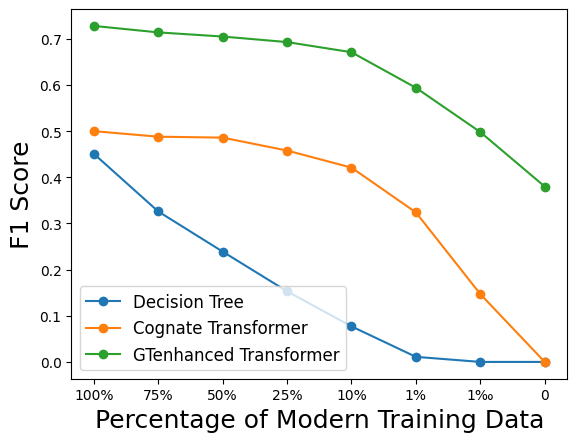
\includegraphics[width=0.35\textwidth]{images/target_reduced.png}
    \caption{Model performance on evaluation with reduced training data from the reconstructed era.}
    \label{fig:reduce input data}
\end{figure}

\begin{table*}[ht]
    \centering
    \footnotesize
    \begin{tabular}{l c c c c c c c c}
    \hline
    \textbf{Model} & \textbf{100\%}  & \textbf{75\%} & \textbf{50\%} & \textbf{25\%} & \textbf{10\%} & \textbf{1\%} & \textbf{1\textperthousand} & 0 \\
    \hline
    Decision Tree & 0.451 & 0.326 & 0.239 & 0.153 & 0.077 & 0.011 & 0 & 0\\
    Cognate Transformer & 0.500 & 0.488 & 0.486 & 0.458 & 0.421 & 0.324 & 0.147 & 0\\
    GTenhanced Transformer & \textbf{0.728} & \textbf{0.714} & \textbf{0.705} & \textbf{0.693} & \textbf{0.671} & \textbf{0.594} & \textbf{0.498} & \textbf{0.380}\\
    \hline
    \end{tabular}
    \caption{Model performance on Reduced Target Training Data Evaluation (Metrics: F1). The target of the model reconstruction is Modern pronunciation. The value of the header represent the percentages of Modern pronunciation data in the training set relative to the entire training set. The division between the training and testing sets follows the phonetic distinction evaluation.}
    %\KZ{Need to explain the zeros in the table.}
    \label{tab:reduce input data}
\end{table*}

\paragraph{Evaluation with Reduced Historical Training Data}

As shown in \figref{fig:reduce history context}, we progressively reduce the historical context data when reconstructing Modern pronunciation. The F1 score decreases more slowly compared to reconstructing MiddleTang pronunciation. Specifically, when reconstructing Modern pronunciation, the F1 score drops from 0.380 to 0.285 as we reduce the available historical context from T+L+S+Y+Q to only T. On the other hand, when reconstructing MiddleTang pronunciation, the F1 score drops from 0.682 to 0.283 as we reduce the historical context from L+S+Y+Q+M to only M. The F1 scores become nearly identical at the final stages. This phenomenon stems from the model's heavier reliance on phonetic information and attention weights from adjacent eras, particularly MiddleTang, LateTang, and Song periods, which exhibit structured and rule-based phonetic patterns.

Additionally, the decline in F1 scores also validates the effectiveness of our dataset. As we reduce the historical context, the model's performance drops, indicating that the available historical phonetic information is crucial for accurate pronunciation reconstruction.

\begin{figure}[ht]
    \centering
    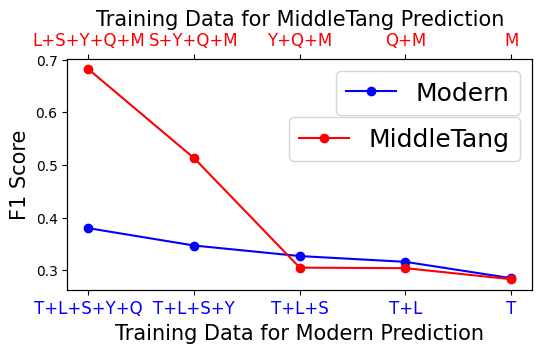
\includegraphics[width=0.35\textwidth]{images/history_reduced.png}
    \caption{Model performance on evaluation with reduced historical training data.}
    \label{fig:reduce history context}
\end{figure}

\paragraph{Predict Future Pronunciations}
Our model has demonstrated robust performance, maintaining a certain level of F1 score even in the absence of training data for specific historical periods. To further explore the capabilities of our model, we conducted an intriguing experiment to predict the pronunciation of Chinese characters in AD 2300\footnote{You can listen to the audio representations of future Chinese pronunciations at the following address: \href{http://47.97.123.246:8080/}{Predict Future Pronunciations Demo}}.
%\href{47.97.123.246:8080}{Future Chinese Pronunciation Demo}
% !TEX root = ../main.tex

\section{Related Work}
%In this section, we review related works covering three aspects, namely using LLMs on mental health, general benchmarks and specific mental health benchmarks.
\paragraph*{LLMs on Mental Health}
Currently, there is relatively limited research utilizing LLMs in the field of mental health. Some studies have delved into the capabilities of LLMs for sentiment analysis and emotion reasoning ~\cite{kocon2023chatgpt, qin2023chatgpt, zhong2023can}. Lamichhane~\cite{Lamichhane2023chatgptapp}, Amin et al. ~\cite{amin2023will}, and Yang et al.~\cite{yang2023evaluations} conducted assessments of ChatGPT's performance across various classification tasks, including stress, depression, and suicide detection. The findings indicate that ChatGPT demonstrates initial potential for mental health applications, yet there remains significant room for improvement.

\paragraph*{General Benchmarks for LLMs}
To evaluate the performance of LLMs across different tasks, several benchmarks have been proposed. C-EVAL~\cite{huang2023ceval} assesses the advanced knowledge and reasoning capabilities of foundation models in Chinese. AGI-Eval~\cite{zhong2023agieval} serves as an evaluation framework for assessing the performance of foundation models in human-centric standardized exams. MMLU~\cite{hendrycks2021measuring} aims to develop a comprehensive test for evaluating text models in multi-task contexts. Big-Bench~\cite{srivastava2023beyond} introduces 204 challenging tasks covering various domains, aiming to evaluate tasks beyond the capabilities of existing language models. HELM ~\cite{helm2023liang} offers a comprehensive assessment, evaluating LLMs across various aspects, such as language understanding and common-sense reasoning. 
These benchmarks, while diverse and comprehensive, primarily emphasize general capabilities and do not cater specifically to the intricacies of mental health.

\paragraph*{Mental Health Benchmarks for LLMs}
Apart from general tasks, specific benchmarks are designed for certain downstream tasks. MultiMedQA~\cite{singhal2023large} focuses on medical question-answering, evaluating LLMs in terms of clinical knowledge and QA abilities. Mental-LLM~\cite{xu2023leveraging} focuses on evaluating the ability of LLMs to predict mental health outcomes through the analysis of online text data. Dialogue safety~\cite{qiu2023benchmark} focuses on the understanding of the safety of responses generated by LLMs in the context of mental health support. Compared to these benchmarks, PsyEval (1) provides a more targeted and comprehensive evaluation of LLMs' capabilities in addressing the unique challenges and nuances of mental health-related tasks. (2) fully considers the differences between the field of mental health and other disciplines.
However, these benchmarks, while addressing specific aspects of mental health or related fields, do not fully encompass the multifaceted nature of mental health issues.

%Contrastingly, our proposed PsyEval benchmark distinguishes itself by offering a more targeted and comprehensive evaluation, specifically designed for mental health-related tasks. PsyEval goes beyond assessing basic understanding or response safety, delving into the complexities unique to mental health. It recognizes that symptoms of mental disorders are subtle, subjective, and highly individualized, requiring a level of expertise, empathy, and emergency response awareness that is not addressed in other benchmarks. This includes understanding nuanced emotional states, detecting subtle signs of mental distress, and providing safe, empathetic interactions. PsyEval, therefore, fills a critical gap in the evaluation of LLMs, positioning itself as a necessary tool for advancing LLMs in the nuanced field of mental health, and setting a new standard for benchmarks in this domain.
%\section{Future Work}
%%To this end, we have successfully built a system
%%which can solve the top-$k$ extraction problem
%%with adequate accuracy and efficiency.
%%With the big data experiment result,
%%we have built a top-$k$ database with
%%over 1.7 million top-$k$ lists of 92.0\% precision.
%%In the future, we will mainly focus on three aspects of work.
%
%The first One is to further enrich the top-$k$ database
%and improve its quality. On the one hand,
%we can use larger training data and
%more sophisticated machine learning models to
%upgrade the system performance;
%on the other hand, we can explore the other source
%of top-$k$ lists rather than top-$k$ pages.
%The slide-show pages can be a good candidate (e.g. Fig. \ref{fig:slideshow}),
%as the top-$k$ list spans across a set of pages, which are connected one another
%by hyperlinks. Intuitively, we can develop a crawler that goes through
%``Previous'' and ``Next'' links and obtain a slide-show page chain.
%But the main challenge is we can not run it on big data as the web snapshot
%cannot support random access (access by URL).
%Furthermore, the snapshot may lose some nodes in a page chain,
%thus we cannot extract the complete list.
%
%The second is to further understand top-$k$ lists, especially the top-$k$ titles.
%In Section \ref{sec:problem}, we define a function $tr$ to convert a textual title
%into a five-tuple representation, which is implemented by Title Classifier.
%However, this representation remains rough as we miss some modifiers other than time and location.
%For example, ``top 10 NBA players alive'' is different from ``top 10 NBA players who have a ring'',
%but they will share the same representation. We may need to include those modifiers in the representation,
%and redefine $tr$ as $tr : (t, d) \rightarrow \mathcal{R} = (k, c, \alpha,
%\mathcal{M})$ where $\mathcal{M}$ is a set of modifiers including the temporal modifier $\tau$ and
%spatial modifier $\sigma$. To do this, we need to improve our Title Classifier to recognize general modifiers,
%probably using the same technology.
%A harder challenge is to calculate semantical similarity between $\mathcal{R}$.
%%which can be defined as $sim : (\mathcal{R_1}, \mathcal{R_2}) \rightarrow score$.
%To solve this, we need to find out the similarity of each part
%($sim_c(c_1, c_2)$, $sim_\alpha(\alpha_1, \alpha_2)$ and $sim_\mathcal{M}(\mathcal{M}_1, \mathcal{M}_2)$)
%and develop a equation/model $sim : (sim_c, sim_\alpha, sim_\mathcal{M}) \rightarrow score$.
%With this function, we can cluster the top-$k$ lists into groups of similar semantics.
%
%The last is to utilize the top-$k$ database.
%As we discuss in Section \ref{sec:intro},
%we attempt to build a Q/A system.
%%which,
%%according to different type of queries,
%%return an instance (e.g. ``Who is the second tallest building in Beijing'') or
%%a ranked list (e.g. ``top 10 richest people in 2010'').
%Given a query $q$, we can first parse it into the tuple representation $\mathcal{R}_q=(k_q,...)$ and
%find a most similar group $g$ from the database.
%To generate a $k_q$-items ranked list (or the $k_q$th item) from $g$, there are two possible solutions.
%The list-wise approach is to (1) rank the lists in $g$ which contain more than $k_q$ items,
%and (2) return the first $k_q$ items (or the $k_q$th item) of the best list.
%The item-wise approach is to merge top-$k$ lists in a group into a bigger one,
%where the main challenge is to calculate the ranking score of each item over aggregation (of ranked lists)
%as an item can exists in multiple top-$k$ lists with different position(ranking within the list).
%This problem is popular in the area of top-$k$ query processing
%as some algorithms are proposed to solve it in different scenarios
%\cite{angel2009ranking,chakrabarti2006ranking,bansal2008ad}.
%In general, we need
%
%
%To obtain the ranking score of each item $i$,
%we need to calculate the score $s_i$ wrt. each list $L_i$ that contains $i$
%(which should be a function of item position $p_i$ and the list size $|L_i|$).
%
%
%We can first define a function $rp: (k, n) \rightarrow score$,
%which gives the score of the $n$th item in any top-$k$ list.
%Then for a instance $i$, assuming it
%
%
%%.
%%The main challenge is to calculate the ranking of each item over aggregation of lists,
%%while a similar problem in the area of top-$k$ query processing
%
%For a list item $i$, it may appears in different list $L$
%The final solution may be a hybrid of the two approach above.



\section{Conclusion}
\label{sec:conclusion}
This paper presents a novel and interesting problem of extracting
top-$k$ lists from the web.  Compared to other structured data,
top-$k$ lists are cleaner, easier to understand and more
interesting for human consumption, and therefore are an important
source for data mining and knowledge discovery. We demonstrate a
algorithm that automatically extracts over 1.7 million such lists from
the a web snapshot and also discovers the structure of each list.  Our
evaluation results show that the algorithm achieves 92.0\% precision
and 72.3\% recall.

%\ZZX{
%In the future, we will focus on building a Q/A system based on
%the large number of top-$k$ lists we extracted.
%%According to different type of queries,
%%the system should return
%%a $k$-item ranked list or the $k$th instance, where $k$ is specified in the query.
%As a top-$k$ query processing system, 
%the main challenge lies in how to generate a $k$-item ranked list 
%from all top-$k$ lists that matches the query.
%Basically we can return the first $k$ items from the best-matching list 
%that contains more than $k$ items.
%A more complicated approach is to merge top-$k$ lists in a group into a bigger one,
%where we need to calculate the ranking score of each item over aggregation (of ranked lists)
%\cite{fagin2001optimal,angel2009ranking,chakrabarti2006ranking}.
%The final solution may be a hybrid of the two approaches above.
%}
%
%Ideally, we should first cluster the top-$k$ lists into groups of similar semantics
%and find out the group $g$ that match the query best.
%To generate a $k$-items ranked list (or the $k$th item) from the group, there are two possible solutions.
%The list-wise approach is to rank the lists in $g$ which contain more than $k$ items,
%and return the first $k$ items (or the $k$th item) of the best list.
%The item-wise approach is to merge top-$k$ lists in a group into a bigger one,
%where is to calculate the ranking score of each item over aggregation (of ranked lists)
%\cite{angel2009ranking,chakrabarti2006ranking,bansal2008ad}.
%The final solution may be a hybrid of the two approaches above.
%}
%
%The format of query is similar to a top-$k$ title,
%which can be represent as a 5-tuple as well
%(e.g. ``Who is the second tallest building in Beijing'' can be represent as (2, building, tallest, in Beijing, none)).
%And the system should return a $k$-item ranked list (or the $k$th item) as answer.
%There are two possible solutions.
%The list-wise approach is to find a best-fitting top-$k$ list according to the query,
%that contains no less than $k$ items.
%The item-wise approach is to cluster the top-$k$ lists into groups of similar semantics.
%and aggregate top-$k$ lists in a group into a bigger ranked list.
%Then given a query, we can find the best-fitting group and return the first $k$ items in the bigger list.
%The final solution may be a hybrid of the two approach above.

%According to different type of queries,
%the system should return an instance (e.g. ``Who is the second tallest building in Beijing'') or
%a ranked list (e.g. ``top 10 richest people in 2010'').
%There are two possible solutions.
%The list-wise approach

\section{Limitations}
In our study, there are some limitations that could be addressed in future research:
\begin{enumerate}
    \item Although the causal relationships between life events and symptoms we identified achieved good results in downstream tasks, and we considered as many common and impactful life events as possible, the 11 categories life events we selected might not cover all events that could potentially affect mental health in life. 
    \item In addition to studying the causal relationships between life events and symptoms, as well as between symptoms themselves, we could also consider other factors and their causal relationships with mental disorders and symptoms. 
    \item Exploration of other downstream tasks involving temporal analysis of mental disorders is necessary. We identified diagnosis point detection and early risk detection here while more tasks can benefit from causal relations.
\end{enumerate}


% (, the 11 categories life events \KZ{Is it 11 categories?} we selected do not cover all events that could potentially affect mental health in life. Achieving this is extremely challenging). 
%Furthermore, 
% \KZ{As a pioneer study, we don't really have to consider all the possible life events.}

%In the downstream task of diagnosis point detection (DPD), we used the RuLSIF\cite{Liu2013Change} model as our baseline, which is a well-established classical model for change point detection (CPD). However, with the rapid development in the CPD field, many models with superior performance have emerged, which might show better results in our task.
%\section*{Acknowledgements}

% Bibliography entries for the entire Anthology, followed by custom entries
%\bibliography{anthology,custom}
% Custom bibliography entries only
\bibliography{custom}

\appendix

\section{Depression Templates}

\begin{table}[htbp]
  \small
  \centering
  \begin{tabular}{l|l}
  \hline
  Dimension & Template \\
  \hline
  Feeling Depressed  &  I feel depressed. \\
  Diagnosis &  I am diagnosed with depression. \\
  Treatment &  I am treating my depression. \\
  \hline
  Sadness & I feel sad.  \\
  Pessimism & I am discouraged about my future.  \\
  Past Failure & I always fail. \\
  Loss of Pleasure & I don't get pleasure from things. \\
  Guilty Feelings & I feel quite guilty. \\
  Punishment Feelings & I expected to be punished. \\
  Self-Dislike & I am disappointed in myself. \\
  Self-Criticalness & I always criticize myself for my faults. \\
  Suicidal Thoughts or Wishes & I have thoughts of killing myself. \\
  Crying & I always cry. \\
  Agitation & I am hard to stay still. \\
  Loss of Interest & It's hard to get interested in things. \\
  Indecisiveness & I have trouble making decisions. \\
  Worthlessness & I feel worthless. \\
  Loss of Energy & I don't have energy to do things. \\
  Changes in Sleeping Pattern & I have changes in my sleeping pattern. \\
  Irritability & I am always irritable. \\
  Changes in Appetite & I have changes in my appetite. \\
  Concentration Difficulty & I feel hard to concentrate on things. \\
  Tiredness  & I am too tired to do things. \\
  Loss of Interest in Sex & I have lost my interest in sex. \\
  \hline
  \end{tabular}
  \caption{The main templates and their corresponding dimensions we used in our experiments, including 3 direct depression descriptions and 21 indirect symptoms derived from BDI-II \citep{beck1996beck}. }
  \label{table:bdi}
\end{table}


We provide the complete templates in Table \ref{table:bdi}. We mainly use a combination of 3 direct depression descriptions and the 21 indirect symptoms derived from BDI-II. We also experimented other well-known depression scales like HDRS \citep{hamilton1986hamilton}, CES-D \citep{Lenore1977CES-D} and PHQ-9 \citep{kroenke2001phq} (We will release our revised templates for theses scales along with our code). The original scales usually contain different descriptions under the same dimension to distinguish different level of intensity or frequency. However, we find that current sentence representations have difficulty in capturing such nuanced differences. We thus condense the descriptions of each dimension into one general template (A few may have more, if there are significant intra-dimension difference).


\end{document}
